\section{Evaluation}
\subsection{Evaluation Setup}
\textbf{Datasets.} We use two benchmark datasets for mobile agents: \textbf{DroidTask} \citep{wen2024autodroid} and \textbf{AndroidLab} \citep{xu2024androidlab}. The DroidTask dataset consists of 158 tasks across 13 basic apps such as Calendar, Clock, Dialer, and others. After filtering out tasks with compatibility issues, we obtain 143 tasks from 12 compatible apps. Some task instructions are revised for clarity while preserving their original intent. The AndroidLab dataset contains more challenging tasks in apps with more complex UI lauyouts, such as Maps, Music, and Zoom. We take all the 98 operation tasks across 9 apps. 

\textbf{Metrics.} Our evaluation focuses on three key aspects: task accuracy, UI exposure reduction, and the costs. These are measured by the following metrics.

\textit{Task Success Rate.} 
We strictly follow the official evaluation criteria provided by each dataset to assess task completion. For Droidtask, a task is considered successful if the human-annotate action sequence is a subsequence of the actions executed by the agent. For AndroidLab, each task defines one or more key states that must be reached or triggered for successful completion. We extract key UI elements from these key states and check whether the agent’s execution process covers these elements in the XML of any visited screen. A task is marked as successful if all required key elements are observed during execution. The success rate is the percentage of successfully completed tasks.

\textit{Reduction Rate.} 
We measure the reduction in UI elements uploaded to the cloud compared to a GPT-4o baseline. To ensure fairness, we consider only the rounds where both methods make the same decision on the same UI screen. Let $E_{\text{GPT-4o}}$ denote the number of UI elements required by the GPT-4o baseline, and let $E_{\text{ours}}$ denote the number required by our design under the same condition. The reduction rate is calculated as:
\begin{equation}
\text{Reduction Rate} = \frac{E_{\text{GPT-4o}} - E_{\text{ours}}}{E_{\text{GPT-4o}}}.
\end{equation}
In addition to evaluating all uploaded elements, the same reduction metric is also computed specifically for sensitive elements, whose sensitivity is determined by another LLM, Qwen2.5-Max.
For completeness, we also provide other reduction metrics under alternative comparison settings in the Appendix~\ref{sec:appendix-more-metrics}.

\textit{Latency and Cloud LLM Token Usage.} Since the overall latency bottleneck lies in the reasoning phase rather than in action execution, we report the total inference time of LLM. For our design, which integrates both local and cloud-based LLMs, we provide separate inference latency for each. To reflect the associated financial cost, we also report the total token usage, including both input and output tokens, for GPT-4o API calls.

\textbf{Baselines.} 
To demonstrate our design's balance between task accuracy and UI exposure reduction, as well as the necessity of cloud–local collaboration, we compare against the following baselines.

\textit{Cloud-Only Baseline.} This baseline follows the mainstream workflow of mobile agent, like AutoDroid \citep{wen2024autodroid}, as shown in Section~\ref{Problem Formulation}, and is powered solely by a cloud-based LLM (e.g., GPT-4o), benefiting from strong reasoning capabilities and typically achieving high task success rates. However, the full UI needs to be uploaded to the cloud at every step. Built on full UI context, this baseline serves as the upper bound for task accuracy, but comes with the highest UI exposure.

\textit{Local-Only Baseline.} This baseline calls only a locally deployable LLM and does not transmit UI to the cloud, which serves as the upper bound for UI exposure reduction (i.e., 100\%), but suffers from significantly lower task success rate.

\textit{Basic-Order Ranking.} It is a variant of our design by replacing the local LLM’s intelligent block ranking with ranking UI blocks in a fixed order (e.g., top to bottom or left to right), mimicking natural human reading behavior. The cloud LLM sequentially receives and accumulates blocks in this basic order until it can make a confident decision. This baseline reflects a trivial rule-based filtering strategy that does not involve local LLM.

\textit{Random Ranking.} It is another variant of our design by ranking and sending UI blocks in a random order to the cloud. 


\textbf{Implementation Details.} For the cloud LLM, we use GPT-4o-2024-11-20 \citep{hurst2024gpt} accessed via OpenAI’s official API. For the local LLMs, we deploy quantized versions of Gemma2-9B-Instruct \citep{team2024gemma}, Qwen2.5-7B-Instruct \citep{yang2024qwen2}, and LLaMA3.1-8B-Instruct \citep{grattafiori2024llama} using Ollama \citep{ollama}, running on a consumer-grade NVIDIA GeForce RTX 4090D GPU. For mobile agent execution environments, we use a real Honor Play3 smartphone with Android 9 for the Droidtask dataset, and the official Pixel 7 Pro emulator with Android 13 from AndroidLab for its dataset. UI states are extracted as XML files using uiautomator2 \citep{uiautomator2} for decision making, and actions are executed in the mobile environment via Android Debug Bridge (ADB) \citep{adb}. For both cloud-only and local-only baselines, we adopt the same prompt configurations as used in AutoDroid \citep{wen2024autodroid}.

\subsection{Main Results and Analysis}
\begin{table}[htbp]
  \caption{Our design vs. Baselines from task success rate and UI exposure reduction rate.}
  \label{main-results}
  \centering
  \resizebox{\columnwidth}{!}{
  \begin{tabular}{ccccccc}
    \toprule
    \multirow{2.5}{*}{\bf Methods} & \multicolumn{2}{c}{\bf DroidTask Dataset} & \multicolumn{2}{c}{\bf AndroidLab Dataset}                 \\
    \cmidrule(r){2-3} \cmidrule(r){4-5} 
    & \bf{Success Rate} & {\bf Reduction Rate} & \bf{Success Rate} & {\bf Reduction Rate}\\
    \midrule
    GPT-4o Baseline      & {\bf 74.13\%} & 0.00\%   & {\bf 44.90\%}   & 0.00\%\\
    \midrule
    Gemma 2-9B Baseline       & 32.87\% & {\bf 100.00\%} & 17.35\% & {\bf 100.00\%}\\
    Qwen 2.5-7B Baseline        & 14.69\% & {\bf 100.00\%} & 5.10\%   & {\bf 100.00\%}\\
    LLaMA 3.1-8B Baseline       & 9.79\%  & {\bf 100.00\%} & 11.22\%   & {\bf 100.00\%}\\
    \midrule
    Ours (GPT-4o + Gemma 2-9B)   & {\bf 69.23\%} & {\bf 55.60\%}  & 37.76\%   & {\bf 34.96\%}\\
    Ours (GPT-4o + Qwen 2.5-7B)  & 61.54\% & 41.89\%  & {\bf 41.84\%}   & 29.97\%\\
    Ours (GPT-4o + LLaMA 3.1-8B) & 49.65\% &40.56\%  & 34.69\%   & 31.65\%\\
    \bottomrule
  \end{tabular}
  }
\end{table}

\textbf{Comparisons with Baselines.}
As shown by Table~\ref{main-results}, the GPT-4o baseline achieves the highest success rate with 0\% UI exposure reduction, while local-only baselines perform significantly worse but achieve 100\% reduction by avoiding any cloud uploads. Our design strikes a balance between these baselines. For the Droidtask dataset, the best 4o \& Gemma combination achieves a 55.6\% reduction with only a 4.9\% drop in success rate compared to the GPT-4o baseline, while outperforming the Gemma-only baseline by 36.36\%. For the AndroidLab dataset, the best-performing 4o \& Qwen combination achieves a small 3.06\% drop in success rate compared to GPT-4o, and outperforms the Qwen-only baseline by 36.74\%, with a 29.97\% UI reduction. Our best reduction-focused setting (4o \& Gemma) achieves a 34.96\% exposure reduction, with a 7.14\% drop in success rate, still outperforming the Gemma-only baseline by 20.41\%. Our design combines the strengths of both cloud and local LLMs, selectively transmitting only essential UI elements to the cloud, thereby reducing data exposure while maintaining comparable performance to the cloud-only baseline.

\textbf{Quantitative Privacy Analysis of Sensitive UI Exposure}
To quantitatively evaluate the privacy benefits of our framework, we conducted a detailed analysis of the sensitive information omitted by CORE, comparing the sensitive UI elements uploaded to the cloud by the GPT-4o baseline and by our method (under the configuration GPT-4o \& Gemma 2-9B). We categorized sensitive data into eight major types: 
(1) Identity \& Account (e.g., username, profile); 
(2) Location \& Schedule (e.g., home address, calendar events); 
(3) Contacts \& Communication (e.g., contact information, messages, call logs); 
(4) Media \& Files (e.g., file name, file content); 
(5) Device \& Usage Info (e.g., device ID, storage); 
(6) Behavior \& Preferences (e.g., interests, browsing history, custom settings); 
(7) Finance \& Security (e.g., payments, passwords, transactions); and 
(8) Other Sensitive Information. For each task step, all uploaded UI elements were analyzed using Qwen2.5-max to identify sensitive content and assign each element to the corresponding category.

\begin{table}[htbp]
  \caption{Comparison of uploaded sensitive UI elements between the GPT-4o baseline and our CORE under two datasets.}
  \label{tab:privacy_reduction}
  \centering
  \resizebox{\columnwidth}{!}{
  \begin{tabular}{ccccccc} 
    \toprule
    \multirow{2.5}{*}{\bf Category} & \multicolumn{3}{c}{\bf DroidTask Dataset} & \multicolumn{3}{c}{\bf AndroidLab Dataset}\\
    \cmidrule(r){2-4} \cmidrule(r){5-7} 
     & \bf{GPT-4o} & {\bf CORE} & \bf{Reduction} & \bf{GPT-4o} & {\bf CORE} & \bf{Reduction}\\
    \midrule
    Identity \& Account   & 91 & 50  & 45.05\%   & 189 & 111 &  41.27\%\\
    Location \& Schedule  & 226 & 70  & 69.03\%   & 299 & 114 & 61.87\%\\
    Contacts \& Communication & 458 & 122  & 73.36\%   & 273 & 203 &25.64\%\\
    Media \& Files & 147 & 32 & 78.23\% & 12 & 12 & 0.00\%\\
    Device \& Usage Info & 0 & 0 & / & 10 & 5 & 50.00\%\\
    Behavior \& Preferences & 45 & 10 & 77.78\% & 77 & 53 & 31.17\%\\
    Finance \& Security & 2 & 2 & 0.00\% & 102 & 90 & 11.76\%\\
    Other Sensitive Information & 0 & 0 & / & 1 & 1 & 0.00\%\\
    \midrule
    \textbf{Total} & \textbf{969} & \textbf{286} & \textbf{70.49\%} & \textbf{963} & \textbf{589} & \textbf{38.84\%}\\
    \bottomrule
  \end{tabular}
  }
\end{table}

The results in Table~\ref{tab:privacy_reduction} show that CORE significantly reduces the number of sensitive UI elements uploaded to the cloud by 70.49\% on DroidTask and 38.84\% on AndroidLab. These reductions are consistent with the overall element reduction rates (55.60\% and 34.96\%, respectively) reported in the main text, confirming that reducing overall UI exposure effectively lowers privacy risks.

Further manual inspection was conducted to understand the sources of reduction. The key findings indicate that most sensitive data fall into the Location \& Schedule and Contacts \& Communication categories, primarily due to apps such as Calendar, Contacts, and Messenger. Representative cases of the CORE framework are summarized below.
\begin{itemize}
\item In a Calendar task (creating a new event), only the UI context relevant to the new event is uploaded, while previously scheduled events on the screen which may reveal the user’s calendar are omitted.
\item In a Contacts task (updating a phone number), only the phone number field is transmitted, whereas unrelated fields such as email and birthday are excluded.
\item In a Messenger task (sending a message), only the current message block is uploaded to the cloud, with prior chat history kept local.
\end{itemize}
These cases demonstrate that CORE effectively reduces unnecessary sensitive UI exposure, thereby enhancing user privacy, comfort, and trust in mobile agent interactions.

\begin{figure}[htbp]
    \centering
    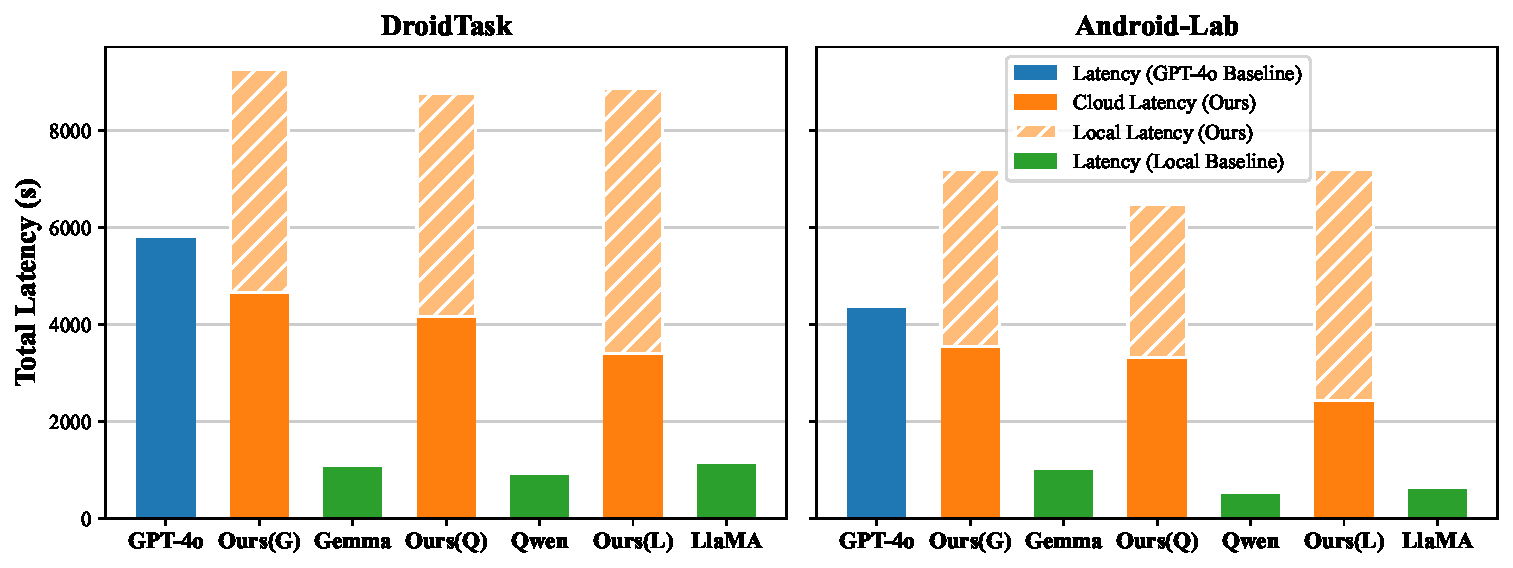
\includegraphics[width=0.63\textwidth]{pics/latency_on_both_new.pdf}
    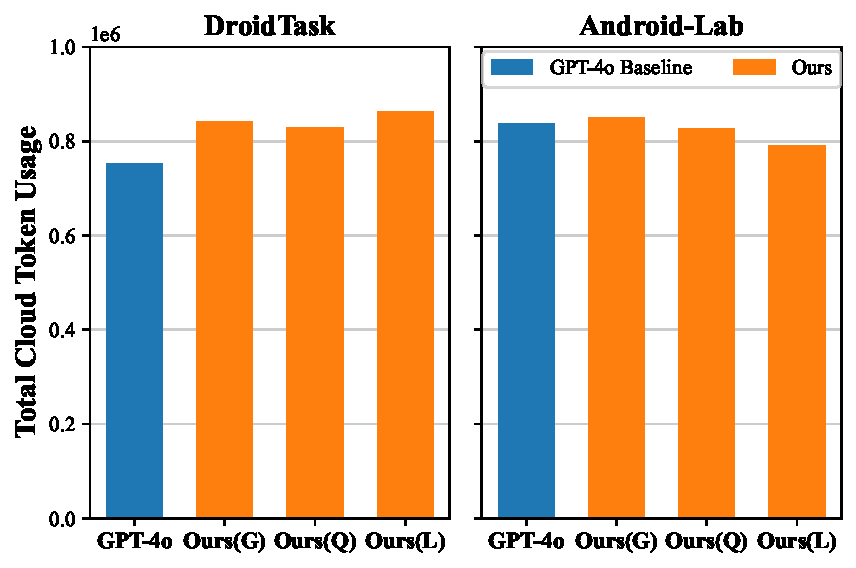
\includegraphics[width=0.36\textwidth]{pics/tokens_on_both_new.pdf}
    \caption{Our design vs. Baselines from latency and cloud LLM token usage.}
    \label{fig:latency_and_tokens}
\end{figure}

\textbf{Cost Analysis.}
Figure~\ref{fig:latency_and_tokens} shows a detailed comparison of latency and cloud LLM token usage between our design with different local LLMs and the baselines. The local baselines yield the lowest latency, but perform too poorly to be considered. Our design reduces cloud inference time by up to 44\% compared to the GPT-4o baseline, because the cloud LLM only needs to deal with the filtered UI content. However, this cloud-local collaborative framework incurs additional overhead on the local side, since the local LLM handles sub-task generation and content filtering. Consequently, the overall latency of our method is \(1.52{\sim}1.61\times\) and \(1.49{\sim}1.66\times\) that of the GPT-4o baseline on DroidTask and AndroidLab, respectively. Regarding cloud LLM token usage, our method consumes \(1.10{\sim}1.15\times\) and \(0.94{\sim}1.01\times\) the tokens of the GPT-4o baseline on the two datasets respectively. Although we substantially reduces the elements uploaded to the cloud, the cloud LLM still incurs token overhead from co-planning and multi-round interactions with the local LLM to accumulate sufficient blocks for co-decision-making. Notably, on the more complex AndroidLab dataset where apps contain many redundant UI elements, the reduced upload volume offsets the extra communication overhead, resulting in a slightly lower overall token cost. Overall, our method achieves a practical trade-off among success rate, upload reduction and cost, with only a slight runtime increase and comparable cloud token usage due to the collaborative design.

\textbf{Impact of Local Model Choice.}
As shown in Table~\ref{main-results}, the performance of our method correlates with the abilities of the local LLM. Gemma2-9B yields the best results among local baselines, followed by Qwen2.5-7B and LLaMA3.1-8B. When combined with GPT-4o in our method, stronger local LLMs lead to higher success and reduction rates, with the Gemma combination achieves near GPT-4o success rate (69.23\%, 37.76\%) with substantial reduction (55.60\%, 34.96\%) on two datasets. Nonetheless, even a weak model like LLaMA, sees substantial gains over its standalone baseline on both datasets(+39.86\%, +23.47\%), confirming the effectiveness of collaboration. Our framework lowers the burden on local LLMs by dividing UI into blocks and avoiding full-screen reasoning. This explains why Qwen, which achieves the lowest 5.10\% success rate as a local baseline on AndroidLab, can reach the highest 41.84\% success rate along with a 29.97\% reduction when paired with GPT-4o.

\textbf{Impact of Dataset Difficulty.}
The two datasets differ significantly in difficulty, as reflected by the cloud LLM performance. The GPT-4o baseline achieves 74.13\% success rate on DroidTask but only 44.90\% on AndroidLab. This is due to differences in apps, task descriptions and minimum steps required. On the relatively easier DroidTask dataset, our method achieves a high success rate of 69.23\% and a reduction rate of 55.60\%. On the more challenging AndroidLab dataset, our 41.84\% success rate remains close to GPT-4o-only performance. Although the reduction rate drops, it still remains around 30\%. This shows that our method generalizes well across tasks of varying complexity.

\textbf{Performance Across different Apps.} 
Figure~\ref{fig:comparison_vertical} presents a detailed per-app comparison of task success rate and UI reduction rate between our method and the GPT-4o baseline on both datasets. As expected, the GPT-4o baseline slightly outperforms our method on most apps (e.g., Gallery, Notes), since it has full access to UI context. Interestingly, we surpass GPT-4o on some apps (e.g., Firefox, Map), largely because we filter out irrelevant UI elements that might distract or mislead the LLM. E.g., complex location data in Map may interfere with reasoning, while our method eliminates such noise and focuses on task-relevant content. Our reduction rates clearly outperform GPT-4o (0\%) but vary across apps, influenced by both task difficulty and UI structure. Simple tasks on Clock require little context, allowing us to aggressively reduce UI elements without sacrificing performance. Apps with flat layouts or unbalanced XML structures (Settings, Pimusic) affect our block partitioning and limit reduction.


\begin{figure}[htbp]
  \centering
  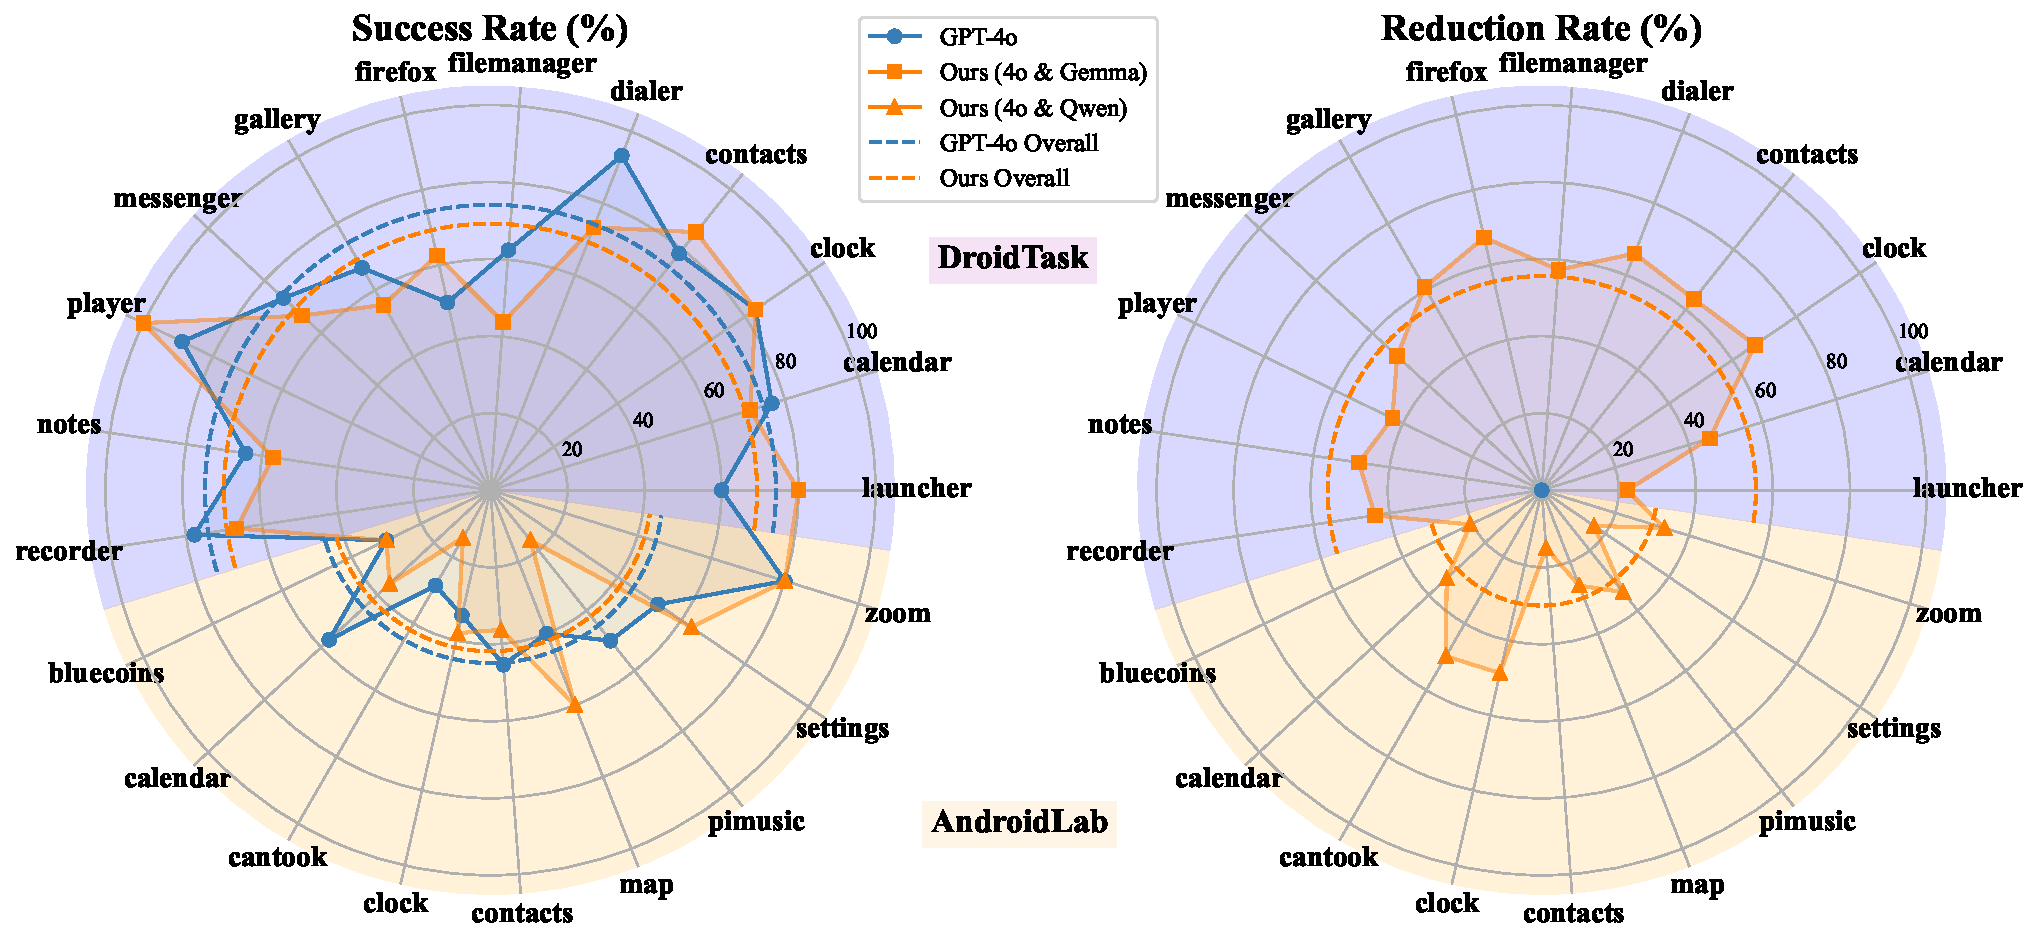
\includegraphics[height=6cm]{pics/radar_chart_sr_upload_colored_labels.pdf}
  \caption{Success and reduction rates of the GPT-4o baseline and our method (using best-performing setting) across apps on both datasets. Note: On the right, GPT-4o appears as a single point due to 0\% reduction. Dashed arcs indicate the overall performance on the entire dataset.}
  \label{fig:comparison_vertical}
\end{figure}

\subsection{Ablation Study}

\begin{table}[htbp]
  \caption{Ablation study results of different design modules over the DroidTask dataset.}
  \label{ablation-results}
  \centering
  \begin{tabular}{ccc|cc}
    \toprule
     & \bf{Success Rate} & \bf{$\Delta$} & {\bf Reduction Rate} & {\bf $\Delta$}\\
    \midrule
    w/o our block partitioning      & 62.24\% & -6.99\%   & 53.44\%   & -2.15\%\\
    w/o our co-planning       & 59.44\% & -9.79\% & 48.67\% & -6.93\%\\
    w/o multi-round interactions         & 36.36\% & -32.87\% & 52.57\%   & -3.03\%\\
    w/o accumulation mechanism          & 53.15\% & -16.08\% & 52.57\%   & -3.03\%\\
    \midrule
    Random ranking        & 51.75\%  & -17.48\% & 35.87\%   & -19.73\%\\
    Basic-order ranking   & 46.15\% & -23.08\%  & 32.59\%   & -23.01\%\\
    \bottomrule
  \end{tabular}
\end{table}

We conduct an ablation study on the DroidTask dataset to isolate the contribution of each module in our collaborative framework. All experiments use the ``Ours (4o \& Gemma)'' setting as the reference.

\textbf{Block Partitioning.} Replacing our XML-layout-informed partitioning with a simple equal split of all UI elements into three groups causes the success rate to drop by 6.99\% and the reduction rate by 2.15\%. This result confirms that leveraging the XML layout to group semantically related elements can help our framework to do better block filtering.

\textbf{Co-planning.} We remove the co-planning module so that no guided sub-tasks are generated collaboratively and the local model must directly rank page blocks on its own. Due to limited planning ability, the local LLM often mis-ranks important blocks on the first pass. These early errors not only reduce accuracy (-9.79\%) but also trigger additional rounds of interaction in the co-decision-making stage, further harming upload reduction (-6.93\%). This ablation underscores the critical role of sub-task co-planning in guiding the local LLM to better rank UI blocks. 

\textbf{Co-decision-making.} Removing multi-round interactions, where the cloud LLM only receives the single top-ranked block from the local LLM without requesting further blocks, causes a 32.87\% drop in success rate and a 3.03\% drop in reduction rate. Similarly, removing the accumulation mechanism (where the cloud LLM, after finding a block inadequate, requests another block from the local model but makes decisions based only on the new block) results in performance decrease (-16.08\% success, -3.03\% reduction). These results demonstrate that our co-decision-making is essential both for mitigating the effects of mis-ranked blocks from the local LLM and for improving the cloud LLM's understanding and decision accuracy on the incomplete page context.

\textbf{Ranking strategies.} Replacing the local LLM's ranking with random ordering reduces success by 17.48\% and reduction by 19.73\%. Using a simple top-to-bottom left-to-right (``basic-order'') block ranking performs even worse (-23.08\% success, -23.01\% reduction). These naive strategies often surface irrelevant blocks unrelated to the task, which not only misleads the cloud model's decisions but also forces additional requests to retrieve more useful blocks. This demonstrates that the local LLM's ranking plays a critical role in efficiently filtering informative content.
